\documentclass[10pt,a4paper]{article}
\usepackage[T1]{fontenc}
\usepackage{lmodern}
\usepackage{amsmath,amssymb,amsthm}
\usepackage{booktabs,array,longtable,graphicx}
\usepackage[margin=2.5cm]{geometry}
\usepackage[hidelinks]{hyperref}

\newtheorem*{lemmaone}{Lemma 1}
\newtheorem*{corone}{Corollary 1}
\newtheorem*{lemmatwo}{Lemma 2}
\newtheorem*{propa}{Proposition 2(a)}
\newtheorem*{propb}{Proposition 2(b)}
\newtheorem*{propproj}{Statement after projection}
\theoremstyle{remark}
\newtheorem*{remark}{Remark}

\newcommand{\F}{\mathcal F^N_\kappa}
\newcommand{\Z}{\mathcal Z}
\newcommand{\hw}{\hat w}
\newcommand{\norm}[1]{\lVert #1\rVert}
\newcommand{\DCE}{$\Delta$-CE}
\newcommand{\TODO}[1]{\par\medskip\noindent\textbf{[#1]}\par\medskip}

\title{Supplementary material for:\\Benchmarking Counterfactual Explanations of Model Change\\with Exact Ground Truth}
\author{Authors as in the main paper}
\date{}

\begin{document}
\maketitle

\noindent This document supplements the main paper. Notation is that of the main paper: $m_o,m_n$ are the margins of $f_{old},f_{new}$, $h=m_n-m_o$, $\kappa$ is the margin, $r$ the budget, $\F=\{z:m_n(z)\le-\kappa,\ m_o(z)\ge\kappa\}$ the set of type-N witnesses, and \DCE{} the nearest witness within $r$. The baselines are CF-diff, Grad-diff, Imp-diff, Seg-search, No-prox and CF-new. Test splits A--D are those of the main paper (Section~\ref{sec:log} lists them with E, F and G). The main paper names its test sets by role: its \emph{main test set} is split A; ``new data'' is split B (hypotheses formed after A), the grid test split, or the further Threshold set C; the registered follow-ups are splits D (unscreened nulls, offsets, ResNet-8), F (learned decoder) and G (two changes at once); the exploratory ResNet-8 test at $\kappa^\star$ is split E. Three more names differ: its \emph{unscreened} nulls are the unfiltered nulls here (admitted without the admission filter), its \emph{filtered CF-new} is the checked counterfactual of Section~\ref{sec:cfcheck}, and in its Table~3 the rows ``$\Delta$-CE $\approx$ Grad-diff, CF-diff'', ``Grad-diff offset-invariant'' and ``No witness on nulls, unscreened; decoder'' are the rows ``Tie'', ``offset-free'' and the two rows for splits D and F here; its column ``Result'' gives the outcome with the earlier codes merged (OSF = reg; pre = pre or grid; post = post or new), which the protocol log gives in full. Its block ``Consistency checks'' holds the three rows that follow from a lemma or the definitions (code D), and ``($\checkmark$)'' marks the rows confirmed at point level only. The $p$ values of that table are Holm-adjusted within three families, each fixed before its data: the grid tests (Grad-diff Recovery $<0.2$ at $\alpha=0$, offset-invariant, rises with $\alpha$, projected $\Delta$-CE $\approx$ Grad-diff on the grid; $m=4$); the tests on new data after split A ($\Delta$-CE $>$ Grad-diff on Threshold, projected $\Delta$-CE $\approx$ Grad-diff on Shortcut; $m=2$); and the logit-offset and locality tests (CF-diff flags $|b|<2\kappa$, normal at $z^\star$ halves the gap; $m=2$). The band tests ($\approx$, offset-invariant) and the halving test use 90\% intervals, all others 95\%.

\section{Proofs}\label{sec:proofs}

The proofs support Lemma~1, Corollary~1, the linear case, Proposition~2 and the statement after projection of the main paper. The closed forms below are for the unbounded case; the experiments use the box $[0,1]^5$, which can change the minimiser. The numerical checks of these formulas (random linear instances, a KKT certificate, an independent SLSQP solve and a CNN sensitivity analysis) are in the repository, in the proofs file and the runs named there.

\subsection{Setting}

The search space is $\Z=\mathbb R^p$ with the Euclidean norm and no box constraints. For a query $z_0$ with label $y$ the margins are $m_o,m_n$ and $h=m_n-m_o$. A query is valid if $m_o(z_0)\ge\kappa$ and $m_n(z_0)\ge\kappa$, with $\kappa>0$. A witness is a point of $\F=\{z:\ m_n(z)\le-\kappa,\ m_o(z)\ge\kappa\}$. The \DCE{} is $z^\star=z_0+u^\star$ with $u^\star\in\arg\min\{\norm u:\ z_0+u\in\F\}$; it is NOT\_FOUND if $\norm{u^\star}>r$.

\subsection{Lemma 1 and Corollary 1}

\begin{lemmaone}
Every witness has $h(z)\le-\kappa-m_o(z)\le-2\kappa$. Hence models whose margins differ by less than $2\kappa$ everywhere have no witness.
\end{lemmaone}
\begin{proof}
At a witness $m_n(z)\le-\kappa$ and $m_o(z)\ge\kappa$, so
\[
h(z)=m_n(z)-m_o(z)\le-\kappa-m_o(z)\le-2\kappa .
\]
If $|h|<2\kappa$ everywhere, no $z$ satisfies this.
\end{proof}

\begin{corone}[constant logit offset]
Let $f_{new}$ add a constant $b$ to the logit of class~1 of $f_{old}$, e.g.\ the prior correction of Saerens et al.\ (2002). Then a type-N witness exists only for the class whose margin $b$ lowers (class~0 if $b>0$, class~1 if $b<0$), only if $|b|\ge2\kappa$, and then exactly at the points with $\kappa\le m_o(z)\le|b|-\kappa$. This set may still be empty in a bounded $\Z$ or beyond the budget $r$. The gradient difference is $\nabla h\equiv0$. No linearity is needed.
\end{corone}
\begin{proof}
The margin of class $y$ is $f_y-f_{1-y}$. Hence for queries with label $y=1$ we have $h\equiv+b$, and for queries with label $y=0$ we have $h\equiv-b$, at every $z$. By Lemma~1 a witness needs $h\le-2\kappa$, which holds on the class whose margin $b$ lowers and requires $|b|\ge2\kappa$. For that class $h\equiv-|b|$, and the witness constraints $m_n=m_o-|b|\le-\kappa$ and $m_o\ge\kappa$ read $\kappa\le m_o(z)\le|b|-\kappa$. Since $h$ is constant, $\nabla h\equiv0$.
\end{proof}

\begin{remark}[the threshold itself]
At $|b|=2\kappa$ the feasible set is the level set $\{m_o=\kappa\}$ of the lowered class: non-empty, but of measure zero. A solver that must land on it exactly finds it only by chance (0 or 1 of 100 points at $|b|=2\kappa$ in the logit-offset experiment). Hence the wording of the main paper, ``once $|b|$ reaches $2\kappa$''.
\end{remark}

\subsection{Linear margins}

Let $m_o(z)=w_o^\top z+b_o$ and $m_n(z)=w_n^\top z+b_n$, with $\rho_o=\norm{w_o}$, $\rho_n=\norm{w_n}$ and $\hw=w/\norm w$. Write
\[
\hw_n=\cos\theta\,\hw_o+\sin\theta\,v,\qquad v\perp\hw_o,\ \norm v=1,\ \theta\in[0,\pi/2),
\]
and define
\begin{itemize}
\item $d_n=(m_n(z_0)+\kappa)/\rho_n>0$, the distance from $z_0$ to $\{m_n=-\kappa\}$;
\item $d_o=(m_o(z_0)-\kappa)/\rho_o\ge0$, the distance from $z_0$ to $\{m_o=\kappa\}$;
\item $d_o'=(m_o(z_0)+\kappa)/\rho_o=d_o+2\kappa/\rho_o$, the distance from $z_0$ to $\{m_o=-\kappa\}$.
\end{itemize}
Factor changes are read in $\Z$ directly. The explanation vectors are:

\begin{center}
\begin{tabular}{@{}>{\raggedright\arraybackslash}p{5.2cm}>{\raggedright\arraybackslash}p{10cm}@{}}
\toprule
Method & Vector\\
\midrule
Witness (\DCE, type N) & $u^\star$\\
Counterfactual differencing (CF-diff) & $u_n-u_o$, with $u_n=-d_n\hw_n$, $u_o=-d_o'\hw_o$ the minimum-norm counterfactuals of each model\\
Gradient difference (Grad-diff; Artelt et al.\ 2021) & $-(\hw_n-\hw_o)$, the normalised margin gradients (constant for linear margins)\\
\bottomrule
\end{tabular}
\end{center}

The witness constraints in $u$ are
\[
\text{(N)}\ \ \hw_n^\top u\le-d_n,\qquad\text{(O)}\ \ \hw_o^\top u\ge-d_o .
\]

\begin{lemmatwo}[the witness for linearly independent normals]
If $\theta\in(0,\pi/2)$ the nearest witness (\DCE) is unique. It is $u_n=-d_n\hw_n$ (the ordinary counterfactual of $f_{new}$) if $u_n$ satisfies (O), i.e.\ if $d_n\cos\theta\le d_o$; otherwise it is the minimum-norm point with both constraints active.
\end{lemmatwo}
\begin{proof}
The feasible set is a non-empty closed convex polyhedron (the normals are independent, so both half-spaces intersect) and $\norm u^2$ is strictly convex, so the minimiser exists and is unique.

(N) is active at the minimiser. Otherwise the minimiser would also minimise $\norm u$ under (O) alone, which gives $u=0$ because $d_o\ge0$; but $u=0$ violates (N) since $d_n>0$.

If (O) is inactive, $u^\star$ minimises $\norm u$ under (N) alone, so $u^\star=u_n$. This is consistent if and only if $u_n$ satisfies (O): $\hw_o^\top u_n=-d_n\cos\theta\ge-d_o$, i.e.\ $d_n\cos\theta\le d_o$.

Otherwise both constraints are active. The KKT conditions put $u^\star$ in $\mathrm{span}\{\hw_o,\hw_n\}$, and the two equalities determine it uniquely there.
\end{proof}

\subsection{Proposition 2(a): offset, $\theta=0$}

\begin{propa}
The gradient difference is $0$; counterfactual differencing is a multiple of $\hw_o$; a witness exists iff $d_n\le d_o$, and then $u^\star=-d_n\hw_o$.
\end{propa}
\begin{proof}
Here $\hw_n=\hw_o=:\hw$.
\begin{enumerate}
\item $\hw_n-\hw_o=0$.
\item $u_n-u_o=(d_o'-d_n)\,\hw$.
\item With $s=\hw^\top u$, (N) reads $s\le-d_n$ and (O) reads $s\ge-d_o$. The feasible set is non-empty iff $d_n\le d_o$. Every feasible $u$ has $\norm u\ge|s|\ge d_n$, with equality only for $u=-d_n\hw$, which is feasible when $d_n\le d_o$.\qedhere
\end{enumerate}
\end{proof}

\begin{remark}
Here $h(z)=(w_n-w_o)^\top z+(b_n-b_o)$ with $w_n=\lambda w_o$, $\lambda=\rho_n/\rho_o$. It is constant only if $\lambda=1$; then $d_n\le d_o\iff h\le-2\kappa$, as in Lemma~1. For $\lambda\ne1$ the condition is on the distances, not on $h$.
\end{remark}

\subsection{Proposition 2(b): rotation, $0<\theta<\pi/2$}

\begin{propb}
(i) The gradient difference has components in the ratio $\tan(\theta/2)<1$ along $(\hw_o,v)$. (ii) The witness satisfies $|u^\star\cdot\hw_o|=\min\{d_n\cos\theta,\ d_o\}$, and its component along $v$ dominates iff $\theta>\pi/4$ or $d_o(\sin\theta+\cos\theta)<d_n$.
\end{propb}
\begin{proof}
Write $u=u_1\hw_o+u_2v+u_\perp$ with $u_\perp\perp\{\hw_o,v\}$. Then (N) reads $u_1\cos\theta+u_2\sin\theta\le-d_n$ and (O) reads $u_1\ge-d_o$.

(i) $\hw_n-\hw_o=(\cos\theta-1)\hw_o+\sin\theta\,v$, and $(1-\cos\theta)/\sin\theta=\tan(\theta/2)<1$.

(ii) The constraints do not involve $u_\perp$, so $u_\perp^\star=0$. By Lemma~2:
\begin{itemize}
\item Case A ($d_n\cos\theta\le d_o$): $u^\star=-d_n\hw_n$, so $u_1^\star=-d_n\cos\theta$ and $u_2^\star=-d_n\sin\theta$.
\item Case B ($d_n\cos\theta>d_o$): $u_1^\star=-d_o$ and $u_2^\star=-(d_n-d_o\cos\theta)/\sin\theta<0$, since $d_n-d_o\cos\theta>d_n(1-\cos^2\theta)>0$.
\end{itemize}
In both cases $|u_1^\star|=\min\{d_n\cos\theta,d_o\}$.

Dominance of $v$ means $|u_2^\star|>|u_1^\star|$. In case A this is $\tan\theta>1$, impossible for $\theta\le\pi/4$. In case B it is
\[
(d_n-d_o\cos\theta)/\sin\theta>d_o\iff d_n>d_o(\sin\theta+\cos\theta).
\]
So for $\theta\le\pi/4$ dominance requires $d_o(\sin\theta+\cos\theta)<d_n$. The condition is also sufficient: for $\theta\le\pi/4$,
\[
(\sin\theta+\cos\theta)\cos\theta-1=\sin\theta(\cos\theta-\sin\theta)\ge0,
\]
so $d_o(\sin\theta+\cos\theta)<d_n$ implies $d_o<d_n\cos\theta$, i.e.\ case B, where it is the dominance condition.

For $\theta>\pi/4$ dominance always holds. In case A, $\tan\theta>1$. In case B, $(\sin\theta+\cos\theta)\cos\theta<1$, so $d_o<d_n\cos\theta<d_n/(\sin\theta+\cos\theta)$, which is the case-B dominance condition. At $\theta=\pi/4$ case A is a tie (not dominance) and $\cos\theta=1/(\sin\theta+\cos\theta)$, so dominance is again $d_o(\sin\theta+\cos\theta)<d_n$. Hence the ``iff'' holds for all $0<\theta<\pi/2$, which is the form stated in the main paper.
\end{proof}

\begin{remark}[budget]
For $\theta\le\pi/4$ a witness dominated by $v$ is in case B with $|u_2^\star|>d_o$, so $\norm{u^\star}>\sqrt2\,d_o$. Within a budget $r$ this needs $d_o<r/\sqrt2$.
\end{remark}

\begin{remark}[counterfactual differencing]
$u_n-u_o=(d_o'-d_n\cos\theta)\hw_o-d_n\sin\theta\,v$.
\end{remark}

\subsection{After projection}

\begin{propproj}
Let $P=I-\hw_o\hw_o^\top$. In case (b) all three explanations are positive multiples of $-v$ (they coincide up to a positive scale). In case (a) they vanish after projection (and the witness may not exist). This is consistent with Theorem~1 of Artelt et al.\ (2021).
\end{propproj}
\begin{proof}
$P\hw_o=0$, $Pv=v$ and $Pu_\perp=u_\perp$. In (b): $P\bigl(-(\hw_n-\hw_o)\bigr)=-\sin\theta\,v$; $Pu^\star=u_2^\star v$ with $u_2^\star<0$ in both cases ($u_\perp^\star=0$); and $P(u_n-u_o)=-d_n\sin\theta\,v$. All point along $-v$. In (a) all three are multiples of $\hw_o$ and project to $0$.
\end{proof}

\begin{remark}[CNNs]
The statement uses one normal $\hw_o$, constant for linear margins. For curved margins the normal at $z_0$ and at $z^\star$ differ; the main paper tests which of the two makes the statement hold approximately (gap at $(z^\star,z_0)$ versus $(z_0,z_0)$).
\end{remark}

\section{Pair-level statistics}\label{sec:pair}

The unit of inference is the \emph{pair} ($f_{old}$, $f_{new}$), not the query point: the 300 points of a pair share one model pair, so point-level intervals do not cover model-to-model variation. All procedures below were fixed before any pair-level number was computed (decision log D-056, S1) and are applied to saved outputs only.
\begin{itemize}
\item \emph{Estimate.} For every row of Table~3 of the main paper, one estimate per pair (the mean over its points); splits are pooled where condition and method agree (A and B).
\item \emph{One-sided tests.} For a claim about a level, an exact one-sided sign test over pairs. For a claim about a difference between two methods, an exact sign-flip permutation test on the pair means, enumerating all $2^n$ sign patterns for $n$ pairs.
\item \emph{Intervals.} A 95\% $t$-interval on the pair means when $n\ge4$; none for $n=3$ (stated as such).
\item \emph{Power floor.} With three pairs the smallest attainable one-sided exact $p$ is $1/8=0.125$, so rows with three pairs cannot reach $p<0.125$ and are reported as not confirmable at pair level.
\item \emph{Sensitivity.} A linear mixed model with a random intercept per pair, for rows with $\ge8$ pairs (details below the table).
\end{itemize}

\begingroup\scriptsize
\setlength{\tabcolsep}{2.5pt}
\begin{longtable}{@{}>{\raggedright\arraybackslash}p{3.8cm}r>{\raggedright\arraybackslash}p{1.9cm}>{\raggedright\arraybackslash}p{2.5cm}>{\raggedright\arraybackslash}p{2.5cm}>{\raggedright\arraybackslash}p{1.2cm}>{\raggedright\arraybackslash}p{2.1cm}@{}}
\caption{Pair-level statistics for the rows of Table~3 of the main paper (exp\_0058, saved outputs only). $n$: pairs; range and mean: per-pair values (Recovery, found-rate or witness share, or a difference); CI: 95\% $t$-interval on the pair means (-- for $n<4$). Exact $p$: ``sign'' is the one-sided exact sign test ($k$ of $n$ pairs on the claimed side); ``flip'' is the exact sign-flip permutation test on the pair means (one-sided for $>0$ claims, two-sided for the $\pm0.10$ band rows, where $k/n$ counts pairs inside the band); ``perm.'' is the Monte Carlo permutation test of the Spearman correlation. Min.\ $p$: smallest value the test can attain with $n$ pairs. MixedLM: intercept (SE) and one-sided Wald $p$ against the row's threshold ($0.9$ for CF-diff, $0.2$ for Grad-diff); for the rotation row, the slope on $\hat\alpha$ (SE) and its two-sided $p$. The MixedLM is a sensitivity check only: with little variance between pairs it treats points as independent, so its $p$ values (down to $10^{-66}$) are far smaller than the pair-level ones and are not evidence at the pair level. Three registered readouts in Table~3 are counts of pairs only: witness $\ge$ margin score $+0.2$ (7 of 8) and, for ResNet-8 on split D, Grad-diff $<0.2$ on offsets and rotation above offset (0 of 3 each).}\label{tab:s1}\\
\toprule
Claim, data & $n$ & Per-pair range & Mean [95\% CI] & Exact $p$ & Min.\ $p$ & MixedLM\\
\midrule
\endfirsthead
\toprule
Claim, data & $n$ & Per-pair range & Mean [95\% CI] & Exact $p$ & Min.\ $p$ & MixedLM\\
\midrule
\endhead
\bottomrule
\endfoot
No witness on nulls, Null, B & 8 & 0.000 to 0.000 & 0.000 [0.000, 0.000] & sign 0.0039 (8/8) & 0.0039 & not fitted (constant 0) \\
No witness on nulls, Adult (MLP) & 5 & 0.000 to 0.000 & 0.000 [0.000, 0.000] & sign 0.0312 (5/5) & 0.0312 & -- \\
No witness on unfiltered nulls, Null, D & 8 & 0.000 to 0.000 & 0.000 [0.000, 0.000] & sign 0.0039 (8/8) & 0.0039 & not fitted (constant 0) \\
No witness on nulls, ResNet-8, D, $\kappa=0.5$ & 2 & 0.890 to 0.910 & 0.900 [--] & sign 1.0000 (0/2) & 0.2500 & -- \\
No witness on nulls, ResNet-8, E, $\kappa^\star=2.5$ & 2 & 0.000 to 0.000 & 0.000 [--] & sign 0.2500 (2/2) & 0.2500 & -- \\
CF-diff (no cut) flags $|b|<2\kappa$, Logit offsets, 12 pairs & 12 & 0.927 to 0.997 & 0.961 [0.947, 0.976] & sign $2.4\times10^{-4}$ (12/12) & $2.4\times10^{-4}$ & 0.961 (0.0066); $1.3\times10^{-20}$ \\
Grad-diff $<0.2$, Grid, $\alpha=0$ & 4 & 0.027 to 0.123 & 0.081 [0.014, 0.148] & sign 0.0625 (4/4) & 0.0625 & -- \\
Grad-diff $<0.2$, Offsets, D & 8 & 0.033 to 0.093 & 0.056 [0.036, 0.076] & sign 0.0039 (8/8) & 0.0039 & 0.056 (0.0084); $1.9\times10^{-66}$ \\
Grad-diff offset-free (difference), Grid, $t$=.60 vs .50, matched by seed & 2 & $-$0.133 to $-$0.063 & $-$0.098 [--] & 1/2 in band; flip 0.5000 (2-sided) & 0.5000 (2-sided) & -- \\
Grad-diff rises with $\alpha$ (contrast), Grid, $\alpha$=.5 vs .1, matched by seed & 2 & 0.537 to 0.603 & 0.570 [--] & sign 0.2500 (2/2); flip 0.2500 & 0.2500 & -- \\
Grad-diff rises with $\alpha$ (rank corr.), Grid, $\alpha>0$ & 24 & 0.163 to 0.937 & 0.629 [0.523, 0.734] & $\rho=0.893$; perm.\ $1.0\times10^{-4}$ & $1.0\times10^{-4}$ (floor) & $\hat\alpha$: 1.374 (0.143); $8.0\times10^{-22}$ \\
$\Delta$-CE $>$ Grad-diff, Threshold, A & 3 & 0.380 to 0.407 & 0.396 [--] & sign 0.1250 (3/3); flip 0.1250 & 0.1250 & -- \\
$\Delta$-CE $>$ Grad-diff, Threshold, B & 3 & 0.270 to 0.360 & 0.312 [--] & sign 0.1250 (3/3); flip 0.1250 & 0.1250 & -- \\
$\Delta$-CE $>$ Grad-diff, Threshold, A+B & 3 & 0.338 to 0.380 & 0.354 [--] & sign 0.1250 (3/3); flip 0.1250 & 0.1250 & -- \\
$\Delta$-CE $>$ Grad-diff, Subgroup, A & 3 & $-$0.123 to $-$0.063 & $-$0.091 [--] & sign 1.0000 (0/3); flip 1.0000 & 0.1250 & -- \\
Tie ($|\Delta|\le0.10$), Shortcut, A & 3 & $-$0.563 to $-$0.507 & $-$0.533 [--] & 0/3 in band; flip 0.2500 (2-sided) & 0.2500 (2-sided) & -- \\
Tie ($|\Delta|\le0.10$), Shortcut, B & 3 & $-$0.593 to $-$0.547 & $-$0.570 [--] & 0/3 in band; flip 0.2500 (2-sided) & 0.2500 (2-sided) & -- \\
Tie ($|\Delta|\le0.10$), Shortcut, A+B & 3 & $-$0.578 to $-$0.527 & $-$0.552 [--] & 0/3 in band; flip 0.2500 (2-sided) & 0.2500 (2-sided) & -- \\
Tie ($|\Delta|\le0.10$), Threshold, A & 3 & 0.380 to 0.407 & 0.396 [--] & 0/3 in band; flip 0.2500 (2-sided) & 0.2500 (2-sided) & -- \\
Tie ($|\Delta|\le0.10$), Threshold, B & 3 & 0.270 to 0.360 & 0.312 [--] & 0/3 in band; flip 0.2500 (2-sided) & 0.2500 (2-sided) & -- \\
Tie ($|\Delta|\le0.10$), Threshold, A+B & 3 & 0.338 to 0.380 & 0.354 [--] & 0/3 in band; flip 0.2500 (2-sided) & 0.2500 (2-sided) & -- \\
Proj.\ $\Delta$-CE $\approx$ Grad-diff ($|\Delta|\le0.10$), Shortcut, B & 3 & $-$0.323 to $-$0.273 & $-$0.304 [--] & 0/3 in band; flip 0.2500 (2-sided) & 0.2500 (2-sided) & -- \\
Proj.\ $\Delta$-CE $\approx$ Grad-diff ($|\Delta|\le0.10$), Grid, 4 pairs & 4 & $-$0.400 to $-$0.307 & $-$0.352 [$-$0.413, $-$0.292] & 0/4 in band; flip 0.1250 (2-sided) & 0.1250 (2-sided) & -- \\
Normal at $z^\star$ halves gap ($T_i>0$), Grid, new, 4 pairs & 4 & 0.011 to 0.268 & 0.119 [$-$0.077, 0.314] & sign 0.0625 (4/4) & 0.0625 & -- \\
\end{longtable}
\endgroup

\paragraph{Method.} The pair (one $f_{old}$ seed with one fine-tuned $f_{new}$) is the unit of inference. For each row one value is formed per pair, the mean over its queries of the quantity named in the main paper. A threshold claim is tested with an exact one-sided sign test over pairs ($k$ of $n$ pairs on the claimed side; pairs equal to the threshold are dropped). A claim about a difference is also tested with an exact sign-flip permutation test on the pair means (all $2^n$ sign patterns). The 95\% intervals are $t$-intervals on the pair means for $n\ge4$, and are not given for $n<4$. The rank correlation of the rotation row is the Spearman $\rho=0.893$ with a one-sided Monte Carlo permutation test (10\,000 permutations within $f_{old}$ seed; floor $1/10\,001$), the same call as in exp\_0047. As a sensitivity analysis, rows with at least 8 pairs are also fitted with a linear mixed model with a random intercept per pair (REML) on the 0/1 point-level outcome (witness found, or Recovery indicator); the rotation row is fitted as Recovery $\sim\hat\alpha+(1\mid\text{pair})$ on 7\,200 points. The null rows have a constant outcome of 0 and are not fitted. For the CF-diff row and the split-D offsets row the optimiser reported that the estimate may lie on the boundary of the parameter space. A two-level bootstrap was not used because it under-covers with few clusters, and a binomial GLMM was not used because \texttt{statsmodels} has no frequentist binomial GLMM; for balanced pairs of 300 points the pair-mean analysis is equivalent.

\paragraph{Pairing and threshold choices recorded with the results.} (i) Splits A and B use the same model pairs on different data; the pooled A+B value of a pair is the mean of its two estimates, so pairs do not accumulate ($n$ stays 3). (ii) For the two grid contrasts (``offset-free'' and ``rises'') the two cells of each contrast are matched by $f_{old}$ seed, giving 2 matched pairs each; the decision log does not fix this matching. (iii) Claimed-side thresholds for the sign test: witness share of null queries $\le0.05$ (the registered per-pair criterion, also for the ResNet-8 rows, where the split-D row has 0 of 2 pairs on the claimed side); CF-diff found-rate $>0.90$ on the 12 logit-offset pairs with $|b|<2\kappa$ ($b\in\{-0.9,-0.5,0.5,0.9\}$, three $f_{old}$ seeds); Grad-diff Recovery $<0.2$; differences $>0$. (iv) The locality row uses, per pair, $T_i=|\mathrm{gap}(z_0,z_0)|-2\,|\mathrm{gap}(z^\star,z_0)|$ on the queries with a witness ($T_i>0$ means the gap narrows by at least half). The registered statistic $T$ uses the pooled gaps, $T=|-0.190|-2\,|0.029|=0.132$, whereas the mean of the $T_i$ is 0.119, because the absolute value is taken per pair before averaging in one case and after averaging in the other.

Rows with $n\le4$ pairs cannot reach $p<0.05$ at the pair level; their point-level confirmations in the main paper (Table~3) rest on the variation between points, not between models.


\section{Sensitivity and alternative metrics}\label{sec:sens}

The numbers in this section are descriptive. They were computed from saved outputs of the locked split A (exp\_0017), the new split B (exp\_0019) and the grid (exp\_0026) by run exp\_0047 (decision log D-052, items E3 and E4); no model or solver was re-run. Methods are named as in the main paper: \DCE{} is type N, and the conditions are Shortcut, Subgroup and Threshold.

\subsection{Budget sensitivity}

The budget $r'$ is varied by thresholding the saved distances, so only $r'\le r$ is computable. Table~\ref{tab:rprime} gives Recovery of \DCE{} on split~A. The last column is the rounded budget $0.54$ used in the exp\_0047 summary; the value of the main paper ($r=0.5413$) differs slightly (Shortcut $0.376$, Subgroup $0.529$, Threshold $0.466$ in Table~2 of the main paper, against $0.373$, $0.528$ and $0.466$ here).

\begin{table}[h]
\caption{Recovery@$r'$ of \DCE{} (type N), split A, mean over three pairs.}\label{tab:rprime}
\centering\small
\begin{tabular}{lccc}
\toprule
 & $r'=0.30$ & $r'=0.40$ & $r'=0.54$\\
\midrule
Shortcut & 0.13 & 0.22 & 0.37 \\
Subgroup & 0.30 & 0.40 & 0.53 \\
Threshold & 0.33 & 0.45 & 0.47 \\
\bottomrule
\end{tabular}
\end{table}

\subsection{Sensitivity to the margin $\kappa$}

Table~\ref{tab:kappa-null} gives the share of null-update queries that have a witness. At $\kappa=0$ the condition is only a sign change, and witnesses appear on most null queries; they disappear by $\kappa=1$ (split A) and the grid null cell is silent at $\kappa=1$. The grid null cell is grid pairs 20 and 21 ($\alpha=0$, $t=0.5$); their realised thresholds $\hat t=0.526$ and $0.464$ mean small real offsets. They are fine-tuned with the recipe of the offsets (10 epochs, learning rate $10^{-3}$), the 8 null pairs of split A with the gentler null recipe (3 epochs, $3\cdot10^{-4}$), which also served the registered nulls of splits D and F. The realised thresholds of the split-A nulls, by the same fit on the same validation points (exp\_0061, D-059, after the results), move by +0.017, +0.035, +0.005, +0.016, +0.004, +0.008, +0.021, +0.010 from $\hat t$ of $f_{old}$ (largest $|\Delta\hat t|=0.035$, $|\hat\alpha|\le0.053$), against $+0.039$ and $-0.032$ for the grid null cell. The threshold shift is thus similar; what differs is the fine-tuning recipe, and $\kappa=0.5$ fits the gentler one. Table~\ref{tab:kappa-rec} gives Recovery and, in brackets, the found-rate by $\kappa$. The found-rate is non-increasing in $\kappa$ in every group (the pre-declared prediction was met). Cells marked n/a were not computed (the split-A analysis used $\kappa\in\{0,0.5,1\}$, the grid variants $\kappa\in\{0,0.25,0.5,1\}$).

\begin{table}[h]
\caption{Share of null queries with a \DCE{} witness (types N or O pooled as saved) by $\kappa$.}\label{tab:kappa-null}
\centering\small
\begin{tabular}{lcccc}
\toprule
 & $\kappa=0$ & $\kappa=0.25$ & $\kappa=0.5$ & $\kappa=1$\\
\midrule
Split A, null pairs 9--16 & 0.83 & n/a & 0.00 & 0.00 \\
Grid null cell (pairs 20, 21) & 0.71 & 0.51 & 0.22 & 0.00 \\
\bottomrule
\end{tabular}
\end{table}

\begin{table}[h]
\caption{Recovery@$r$ of \DCE{} (found-rate in brackets) by $\kappa$. The grid row is the group of pure-offset grid pairs ($\alpha=0$) of exp\_0047; for $\kappa=0.5$ the split-A rows reproduce Table~2 of the main paper.}\label{tab:kappa-rec}
\centering\small
\begin{tabular}{lcccc}
\toprule
 & $\kappa=0$ & $\kappa=0.25$ & $\kappa=0.5$ & $\kappa=1$\\
\midrule
Split A, Shortcut & 0.33 (0.93) & n/a & 0.38 (0.84) & 0.37 (0.71) \\
Split A, Subgroup & 0.37 (0.99) & n/a & 0.53 (0.81) & 0.57 (0.70) \\
Split A, Threshold & 0.46 (0.47) & n/a & 0.47 (0.47) & 0.20 (0.27) \\
Grid, $\alpha=0$ offsets & 0.47 (0.47) & 0.46 (0.47) & 0.35 (0.38) & 0.02 (0.04) \\
\bottomrule
\end{tabular}
\end{table}

\subsection{Rank metrics}

Recovery counts a method only when its largest factor change is $k^\star$. As a check on that single notion, we computed for each point the rank of $k^\star$ in the absolute factor change of each explanation (ties take the worst rank; NOT\_FOUND has reciprocal rank 0) and report the mean reciprocal rank (MRR) and Top-2 (the share of points with $k^\star$ among the two largest changes). For the grid, $k^\star$ is colour when $\alpha>0$ and aspect when $\alpha=0$ with $t\ne0.5$. Table~\ref{tab:rank} lists MRR/Top-2. Seg-search, No-prox and Imp-diff were not computed on the grid groups (n/a).

\begin{table}[h]
\caption{MRR / Top-2 by method and condition (split A and grid groups; exp\_0047).}\label{tab:rank}
\centering\scriptsize
\setlength{\tabcolsep}{3.5pt}
\begin{tabular}{lccccccc}
\toprule
 & $\Delta$-CE & CF-diff & Grad-diff & Imp-diff & Seg-search & No-prox & CF-new\\
\midrule
Split A, Shortcut & 0.59/0.75 & 0.70/0.75 & 0.95/0.98 & 0.50/1.00 & 0.04/0.03 & 0.46/0.48 & 0.48/0.81 \\
Split A, Subgroup & 0.65/0.70 & 0.61/0.75 & 0.78/0.84 & 0.32/0.33 & 0.08/0.09 & 0.40/0.42 & 0.60/0.73 \\
Split A, Threshold & 0.47/0.47 & 0.83/0.88 & 0.36/0.25 & 1.00/1.00 & 0.07/0.08 & 0.35/0.38 & 0.90/0.90 \\
Grid, $\alpha=0$ & 0.30/0.30 & 0.75/0.78 & 0.37/0.30 & n/a & n/a & n/a & 0.96/0.96 \\
Grid, $\alpha=0.1$ & 0.15/0.13 & 0.42/0.35 & 0.58/0.61 & n/a & n/a & n/a & 0.31/0.14 \\
Grid, $\alpha=0.25$ & 0.31/0.39 & 0.56/0.60 & 0.81/0.88 & n/a & n/a & n/a & 0.39/0.51 \\
Grid, $\alpha=0.5$ & 0.53/0.72 & 0.70/0.77 & 0.94/0.97 & n/a & n/a & n/a & 0.45/0.82 \\
\bottomrule
\end{tabular}
\end{table}

The pre-declared prediction was that, within each group, the order of methods by MRR equals the order by Recovery. It was \textbf{not met} in 6 of the 7 groups (it holds for the grid at $\alpha=0.5$ only). In every group the first two methods are the same under both orders; the swaps are among the lower-ranked methods (Imp-diff, CF-new, No-prox, Seg-search, and Grad-diff on Threshold) and, on the grid, \DCE{} falls one place under MRR, because NOT\_FOUND counts as reciprocal rank 0 and so weighs its found-rate more. Table~\ref{tab:order} gives both orders.

\begin{table}[h]
\caption{Order of methods by Recovery and by MRR.}\label{tab:order}
\centering\scriptsize
\setlength{\tabcolsep}{3pt}
\begin{tabular}{@{}l>{\raggedright\arraybackslash}p{5.6cm}>{\raggedright\arraybackslash}p{5.6cm}c@{}}
\toprule
Group & By Recovery & By MRR & Same\\
\midrule
Split A, Shortcut & Grad-diff\,$>$\,CF-diff\,$>$\,$\Delta$-CE\,$>$\,No-prox\,$>$\,CF-new\,$>$\,Seg-search\,$>$\,Imp-diff & Grad-diff\,$>$\,CF-diff\,$>$\,$\Delta$-CE\,$>$\,Imp-diff\,$>$\,CF-new\,$>$\,No-prox\,$>$\,Seg-search & no \\
Split A, Subgroup & Grad-diff\,$>$\,$\Delta$-CE\,$>$\,CF-diff\,$>$\,CF-new\,$>$\,No-prox\,$>$\,Seg-search\,$>$\,Imp-diff & Grad-diff\,$>$\,$\Delta$-CE\,$>$\,CF-diff\,$>$\,CF-new\,$>$\,No-prox\,$>$\,Imp-diff\,$>$\,Seg-search & no \\
Split A, Threshold & Imp-diff\,$>$\,CF-new\,$>$\,CF-diff\,$>$\,$\Delta$-CE\,$>$\,No-prox\,$>$\,Seg-search\,$>$\,Grad-diff & Imp-diff\,$>$\,CF-new\,$>$\,CF-diff\,$>$\,$\Delta$-CE\,$>$\,Grad-diff\,$>$\,No-prox\,$>$\,Seg-search & no \\
Grid, $\alpha=0$ & CF-new\,$>$\,CF-diff\,$>$\,$\Delta$-CE\,$>$\,Grad-diff & CF-new\,$>$\,CF-diff\,$>$\,Grad-diff\,$>$\,$\Delta$-CE & no \\
Grid, $\alpha=0.1$ & Grad-diff\,$>$\,CF-diff\,$>$\,$\Delta$-CE\,$>$\,CF-new & Grad-diff\,$>$\,CF-diff\,$>$\,CF-new\,$>$\,$\Delta$-CE & no \\
Grid, $\alpha=0.25$ & Grad-diff\,$>$\,CF-diff\,$>$\,$\Delta$-CE\,$>$\,CF-new & Grad-diff\,$>$\,CF-diff\,$>$\,CF-new\,$>$\,$\Delta$-CE & no \\
Grid, $\alpha=0.5$ & Grad-diff\,$>$\,CF-diff\,$>$\,$\Delta$-CE\,$>$\,CF-new & Grad-diff\,$>$\,CF-diff\,$>$\,$\Delta$-CE\,$>$\,CF-new & yes \\
\bottomrule
\end{tabular}
\end{table}

\emph{Set-recovery.} Counting a method correct when the two largest changes are $\{$aspect, colour$\}$, on the 24 grid pairs with $\alpha>0$: CF-new 0.49, CF-diff 0.39, $\Delta$-CE 0.37, Grad-diff 0.11.

\section{Computational budget}\label{sec:budget}

All counterfactual methods share one solver and the settings of the Tier~0 configuration (file \texttt{tier0.yaml} in the repository): an Adam phase with $R=5$ restarts of $T=400$ steps, learning rate $0.05$ and initial proximity weight $\lambda_0=1$ halved 8 times; noise $\sigma=0.05$ for the restarts; then an SLSQP polish of at most 100 iterations. The budget is $r=0.5413$, the margin $\kappa=0.5$, and each pair uses 300 valid test points (the ResNet-8 runs use 100 queries per pair and X5 uses 100).

Table~\ref{tab:s5} gives the time per query of each method, from the \texttt{runtime} fields saved with the runs of the main paper. The saved records hold time, not forward or backward pass counts, so no such counts are reported. Wall time is the pair wall time divided by the number of points (the solver ran with parallel workers); CPU time is the solver CPU seconds divided by the number of points; both are shown as mean (min--max) over pairs, in seconds. For the X1 baselines the time is the per-pair total divided by the number of points. Runs were made on different machines, so times are not comparable across runs. n/a: not recorded. The ResNet-8 runs (exp\_0050, exp\_0054) saved no runtime fields.

\begingroup\small
\begin{longtable}{@{}lcc@{}}
\caption{Seconds per query, mean (min--max) over pairs (exp\_0058 S2, saved outputs).}\label{tab:s5}\\
\toprule
Method & Wall s/query & CPU s/query\\
\endfirsthead
\toprule
Method & Wall s/query & CPU s/query\\
\endhead
\midrule
\multicolumn{3}{@{}l}{\emph{A exp\_0017} (17 pairs)}\\
No-prox & 0.656 (0.59--0.835) & 5.17 (4.66--6.59) \\
CF-new & 0.617 (0.548--0.724) & 4.86 (4.3--5.72) \\
$\Delta$-CE, $\kappa=0$ & 2.16 (1.2--9.78) & 13.2 (9.52--17.4) \\
$\Delta$-CE, $\kappa=1$ & 2.54 (1.45--3.41) & 20.2 (11.5--27.1) \\
CF-diff (B1) & 1.27 (1.13--1.47) & 10 (9--11.6) \\
CF-diff (B1-det) & 0.351 (0.31--0.44) & 2.76 (2.41--3.46) \\
Grad-diff & 0.000666 (0.000599--0.000755) & n/a \\
Imp-diff & n/a (total 24.4 per pair) & n/a \\
Seg-search & 0.432 (0.404--0.485) & n/a \\
$\Delta$-CE, type N & 2.42 (1.28--3.31) & 19.1 (10--26.2) \\
$\Delta$-CE, type O & 3.2 (2.96--3.66) & 25.3 (23.6--29.1) \\
\midrule
\multicolumn{3}{@{}l}{\emph{B exp\_0019} (14 pairs)}\\
CF-diff (B1) & 1.25 (1.16--1.3) & n/a \\
CF-diff (B1-det) & 0.341 (0.309--0.373) & n/a \\
Grad-diff & 0.000674 (0.000635--0.000749) & n/a \\
$\Delta$-CE, type N & 4.01 (1.23--23.5) & 20 (9.77--25.6) \\
$\Delta$-CE, type O & 3.1 (2.93--3.24) & 24.6 (23.2--25.6) \\
\midrule
\multicolumn{3}{@{}l}{\emph{grid exp\_0026} (32 pairs)}\\
CF-new & 1.09 (0.558--1.4) & 8.33 (4.34--10.5) \\
CF-diff (B1-det) & 0.641 (0.301--0.853) & n/a \\
Grad-diff & 0.00202 (0.000652--0.0133) & n/a \\
$\Delta$-CE, type N & 4.39 (2.02--23.2) & 29.2 (15.9--47.1) \\
$\Delta$-CE N, $\kappa=0$ & 3.26 (1.67--4.77) & 24.9 (13.1--36.3) \\
$\Delta$-CE N, $\kappa=0.25$ & 3.73 (1.93--5.84) & 28.7 (15.3--43.5) \\
$\Delta$-CE N, $\kappa=1$ & 7.41 (2.71--23.9) & 39.7 (21.5--55.5) \\
\midrule
\multicolumn{3}{@{}l}{\emph{H7 exp\_0032} (30 pairs)}\\
CF-diff (B1-det) & 0.694 (0.368--0.941) & n/a \\
$\Delta$-CE, type N & 5.04 (3.56--6.65) & 37.2 (26.7--51.6) \\
\midrule
\multicolumn{3}{@{}l}{\emph{H8 exp\_0033} (24 pairs)}\\
$\Delta$-CE, type N & 3.91 (1.73--6.73) & 30.5 (13.5--52.8) \\
\midrule
\multicolumn{3}{@{}l}{\emph{D exp\_0049} (17 pairs)}\\
$\Delta$-CE, type N & 10.3 (7.96--11.8) & 40.4 (31.5--46.3) \\
$\Delta$-CE, type O & 11.1 (10.7--11.5) & 43.7 (42.2--45.3) \\
\midrule
\multicolumn{3}{@{}l}{\emph{X1 exp\_0048} (17 pairs)}\\
IG-diff & 0.125 (0.0737--0.148) & n/a \\
SHAP-diff & 4.12 (2.38--4.73) & n/a \\
Imp-diff (adaptation data) & 0.17 (0.0978--0.195) & n/a \\
Seg-search $\times10$ & 9.24 (5.38--11.5) & n/a \\
\midrule
\multicolumn{3}{@{}l}{\emph{ResNet exp\_0050 / exp\_0054}: no runtime fields saved (chunked local run); n/a}\\
\bottomrule
\end{longtable}
\endgroup


\section{Learned latent space (X5)}\label{sec:x5}

\emph{Registration.} The design was registered at \url{https://osf.io/fr7jv} on 2026-11-04, before the autoencoder was trained and before the test data (split F) existed (decision log D-056). The question is whether abstention on null updates and detection of offsets survive when the exact renderer is replaced by the decoder of a VAE learned from images; Lemma~1 holds in any search space, but a decoder can produce off-manifold images on which the two CNNs differ by more than $2\kappa$.

\emph{Fixed elements.}
\begin{itemize}
\item VAE: $32\times32\times3$, two stride-2 convolutions (32 and 64 channels), latent dimension 16, symmetric decoder, BCE and KL with $\beta=1$, 30 epochs, Adam $10^{-3}$, batch 256, seed 11000, trained on 50\,000 clean rendered images. Gate on validation: each $f_{old}$ must classify the decoded reconstructions with accuracy $\ge0.90$; one retrain with $\beta=0.5$ if it fails, otherwise ``did not pass its gate'' and no search.
\item Search in $\mathbb R^{16}$ through the decoder with the solver settings of the split-D run and $\mu\norm z^2$ regularisation ($\mu=0.01$); $\kappa=0.5$; $r_{\mathrm{VAE}}=2\times$ the median distance of ordinary counterfactuals of $f_{new}$ on validation, computed once and locked before split F was generated.
\item Split F: the 8 qualified split-D offsets and the 8 nulls; 100 valid queries per pair (registered fallback; D-056 feasibility), data seed $10500+p$.
\item Primary readout: witness share on the null queries (800 at 100 per pair; 1\,600 as registered at 200), pooled and per pair; prediction $\le0.05$ in both. Descriptive: detection of offsets at the null thresholds for \DCE, CF-diff and margin scores; share of witnesses on the data manifold (inverse-rendering error below the 95\% validation quantile); Recovery with factors read by inverse rendering.
\item No quantity above ($\kappa$, $r_{\mathrm{VAE}}$, $\beta$ beyond the one gate fallback, number of queries, pairs) is changed after any X5 number; all readouts are reported whatever their value.
\end{itemize}

\emph{Execution.} The VAE passed its gate at $\beta=1$ (accuracy of $f_{old}$ seeds 0--4 on reconstructions 0.974--0.985; reconstruction MSE $2.3\cdot10^{-4}$); $r_{\mathrm{VAE}}=1.641$ (200/200 counterfactuals found on validation, median distance 0.820). The registered feasibility rule (24 CPU-hours) was exceeded at 200 queries per pair ($\approx76$ CPU-h) and at 100 ($\approx38$); its last step names a GPU, but the dominant cost (per-point SLSQP in float64) does not run faster on one, so the 100-query configuration ran on four CPU kernels (decided and logged before split F was generated; the only deviation). Runs: exp\_0056 (VAE, gate, $r_{\mathrm{VAE}}$), exp\_0057 (search, analysis).

\emph{Results.} \textbf{No null query has a witness: 0/800, and 0 in each of the 8 null pairs} (prediction met). CF-diff attributes a change to 85--94\% of the same queries. Thresholds from these nulls ($\tau_0$ / $\tau_{5\%}$): $s_M$ 1.136 / 0.624; $s_{M,r}$ 1.384 / 0.972; CF-diff 1.950 / 0.246. Table~\ref{tab:x5} gives detection on the lowered class of the offsets: \DCE{} witnesses exist for at least half of the lowered-class queries in 6 of 8 pairs (prediction $\ge5/8$ met); CF-diff flags none at $\tau_0$ in any pair. The two low pairs (100, 101) were also the lowest on split D in factor space (0.17, 0.20). Of the offset witnesses, 91\% are on the data manifold by the registered criterion (none exist on nulls). Recovery with factors read by inverse rendering (approximate): \DCE{} 0.02--0.46 over all queries (only the lowered class, about half, can have a type-N witness), CF-diff 0.55--0.82.

\begin{table}[h]
\centering\small
\caption{X5: share of lowered-class (class 1) queries flagged, thresholds set on the X5 nulls.}\label{tab:x5}
\begin{tabular}{lccccccc}
\toprule
Pair ($t$, seed) & $n$ & \DCE & $s_M$ $\tau_0$ & $s_M$ $\tau_{5\%}$ & $s_{M,r}$ $\tau_0$ & CF-diff $\tau_0$ & CF-diff $\tau_{5\%}$\\
\midrule
100 (.53, 2) & 60 & 0.12 & 0.00 & 0.03 & 0.00 & 0.00 & 0.12\\
101 (.56, 2) & 54 & 0.13 & 0.00 & 0.09 & 0.00 & 0.00 & 0.06\\
102 (.60, 2) & 48 & 0.85 & 0.02 & 0.21 & 0.06 & 0.00 & 0.25\\
104 (.56, 3) & 56 & 0.66 & 0.00 & 0.23 & 0.11 & 0.00 & 0.21\\
105 (.60, 3) & 46 & 0.96 & 0.00 & 0.20 & 0.17 & 0.00 & 0.35\\
106 (.53, 4) & 48 & 0.98 & 0.48 & 0.98 & 0.77 & 0.00 & 0.52\\
107 (.56, 4) & 53 & 0.91 & 0.36 & 0.89 & 0.66 & 0.00 & 0.34\\
108 (.60, 4) & 43 & 0.95 & 0.58 & 0.93 & 0.91 & 0.00 & 0.84\\
\bottomrule
\end{tabular}
\end{table}

\emph{Scope.} One VAE ($\beta=1$, latent 16) on the same synthetic images; \emph{where} is read approximately; the margin score again tells \emph{whether} at 5\% in the pairs with larger shifts.

\section{Two independent local changes (X6)}\label{sec:x6}

\emph{Registration.} Registered at \url{https://osf.io/fp8uc} on 2026-11-05, before any X6 model was trained and before the test data (split G) existed (decision log D-057). The question is whether the nearest witness points to the change near the query when an update makes two independent changes in different regions.

\emph{Design.} $f_{new}$ is $f_{old}$ fine-tuned on Shortcut data (70\% of samples with aspect in $[0.4,0.6]$, colour agreeing with the noise-free label with probability 0.99) whose labels are then flipped for size $>0.75$, with 5\% label noise; 10 epochs, Adam $10^{-3}$, batch 256. Pairs 130--137: $f_{old}$ seeds 0--4 and 0--2 with a second adaptation draw. Qualification (validation): $\Delta$Flip of colour and of size $\ge0.15$, of background and position $\le0.05$. Test: 300 valid queries per pair (data seed $13000+p$); $\kappa$, $r$ and the solver as in the main paper. Primary readout: among queries with a witness, $L$ = share whose largest $|\Delta\phi|$ is size for queries with size $\ge0.60$ (near the subgroup) minus the same share for size $\le0.45$ (far); prediction $L>0$ in every qualified pair and pooled $L\ge0.30$, exact sign test over pairs.

\emph{Results.} All 8 pairs qualified ($\Delta$Flip colour 0.34--0.45, size 0.29--0.36, background/position $\le0.03$), so the test is confirmatory. \textbf{$L>0$ in 8 of 8 pairs, pooled $L=0.50$, sign test $p=0.0039$} (prediction met). Per pair: 0.59, 0.54, 0.53, 0.23, 0.52, 0.60, 0.50, 0.48; near the subgroup 0.46--0.75 of witnesses change size most, far from it 0.13--0.23; witnesses were found for 0.95--1.00 of queries. Controls (pooled $L$): Grad-diff 0.09, CF-diff 0.13, Imp-diff 0 by construction (one vector per pair), and CF-new 0.51: the counterfactual of $f_{new}$ alone localises as well, with the same top-1 shares and MRR as \DCE{} (Table~\ref{tab:x6}). Where $f_{old}$ keeps its decision at $f_{new}$'s counterfactual, the nearest witness is that counterfactual (for any margins, as in case A of Lemma~2); the witness adds the verified check that $f_{old}$ is unchanged, and it is silent on null updates, where CF-new returns a point for 0.996 of queries (main Table~2). Imp-diff ranks neither colour nor size first in 8 of 8 pairs (prediction met).

\begin{table}[h]
\centering\small
\caption{X6, mean over the 8 pairs. Set-recovery: the two largest $|\Delta\phi|$ are colour and size.}\label{tab:x6}
\begin{tabular}{lccccc}
\toprule
Method & set-recovery & MRR colour & MRR size & top-1 colour & top-1 size\\
\midrule
\DCE & 0.26 & 0.66 & 0.63 & 0.51 & 0.43\\
CF-new & 0.24 & 0.66 & 0.63 & 0.51 & 0.43\\
Grad-diff & 0.15 & 0.51 & 0.62 & 0.29 & 0.39\\
CF-diff & 0.04 & 0.48 & 0.50 & 0.23 & 0.23\\
Imp-diff & 0.00 & 0.42 & 0.33 & 0.00 & 0.00\\
\bottomrule
\end{tabular}
\end{table}

\begin{figure}[ht]
\centering
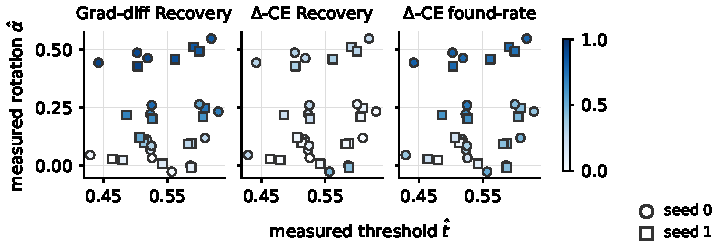
\includegraphics[width=0.8\linewidth]{figures/map_names.pdf}
\caption{Grid pairs placed at the measured rotation $\hat\alpha$ and threshold $\hat t$ of each $f_{new}$: Recovery of Grad-diff and of $\Delta$-CE, and found-rate of $\Delta$-CE (colour scale 0--1). Hollow markers are the pairs of the grid null cell ($\alpha=0$, $t=0.5$), which has no ground-truth factor $k^\star$; marker shape is the seed of $f_{old}$. This figure was Figure~1 of earlier versions of the main paper.}\label{fig:map}
\end{figure}

\section{Witness versus a checked counterfactual (D-059)}\label{sec:cfcheck}

Written after all results were known (second reader's review, 6 Nov), from saved outputs and hash-verified models only (exp\_0061, \texttt{dce.cli.cfnew\_filter}); descriptive, no test. The \emph{checked} counterfactual of $f_{new}$ keeps the saved counterfactual of $f_{new}$ ($m_n\le-\kappa$) only if $m_o\ge\kappa$ there (two forward passes), and is NOT\_FOUND otherwise. Its points are witnesses; the extra witnesses of \DCE{} are at queries where the counterfactual of $f_{new}$ is not one. On the 8 null pairs of split A the checked counterfactual is silent (0/2\,400), like \DCE. In X6 it finds witnesses for 0.87 of queries (\DCE{} 0.98) and localises with pooled $L=0.48$ (\DCE{} 0.50). Null-adjusted Recovery subtracts the rate at which the same method names $k^\star$ on the 8 null pairs.

\begin{table}[h]
\centering\scriptsize
\setlength{\tabcolsep}{3pt}
\caption{Split A, mean of 3 pairs. Found: share of queries with a witness. Rec.: Recovery@$r$. Case B: Recovery of \DCE{} from witnesses the checked counterfactual does not give. Null-adjusted: Recovery minus the rate of naming $k^\star$ on nulls.}\label{tab:cfcheck}
\begin{tabular}{lcccccccccc}
\toprule
& \multicolumn{2}{c}{Found} & \multicolumn{2}{c}{Rec.} & & \multicolumn{5}{c}{Null-adjusted Recovery}\\
Change & \DCE & checked CF & \DCE & checked CF & case B & \DCE & CF-new & Imp-diff & CF-diff & Grad-diff\\
\midrule
Shortcut & 0.84 & 0.42 & 0.38 & 0.03 & 0.35 & +0.38 & +0.07 & +0.00 & +0.44 & +0.79\\
Subgroup & 0.81 & 0.46 & 0.53 & 0.30 & 0.22 & +0.53 & +0.30 & +0.00 & +0.08 & +0.25\\
Threshold & 0.47 & 0.46 & 0.47 & 0.45 & 0.01 & +0.47 & -0.09 & +0.38 & +0.37 & +0.02\\
\bottomrule
\end{tabular}
\end{table}

\section{Protocol log}\label{sec:log}

Table~\ref{tab:splits} lists the test splits of the main paper and when each was formed relative to the results that motivated its tests. Times are local (UTC+7). The rules for each follow-up are in the decision log (\texttt{research/DECISIONS.md}) with dated commits; the OSF registrations are the external timestamps.

\begin{table}[h]
\caption{Test splits and when they were formed. D-xxx: decision-log entry.}\label{tab:splits}
\centering\scriptsize
\setlength{\tabcolsep}{3pt}
\begin{tabular}{@{}l>{\raggedright\arraybackslash}p{2.6cm}>{\raggedright\arraybackslash}p{4.0cm}>{\raggedright\arraybackslash}p{5.2cm}@{}}
\toprule
Split & Run, data & Tests & When formed\\
\midrule
A & exp\_0017; Tier~0 locked test, 5\,000 rendered samples (clean split seed 1234); pairs 0--16 & Main comparison (Table~2), confirmatory & Rules (amendments v1.1--v1.8, D-018 to D-031) committed 15--16 Oct before the run. Run started 16 Oct 23:03, evaluated once (candidate lock; D-011)\\
B & exp\_0019; new Tier~0 test set, factor seed 2027, 5\,000 samples; 300 points per pair (seed $8000+$pair id) & C1--C3 (e.g.\ $\Delta$-CE vs.\ Grad-diff on Threshold, projection, nulls), D-034 & Hypotheses formed after the split-A results; D-034 committed 18 Oct 01:26, run from 18 Oct 01:40 on fresh data\\
C & exp\_0041; \texttt{new\_test\_set}$(9100+\text{pair id})$, seeds 9106--9108, Threshold pairs 6--8, 300 points per pair & Type-N, type-O and union Recovery (descriptive), D-048 & Rules written on 25 Oct, after the split-B results, before the data were generated (commit 8bae341)\\
D & exp\_0049, exp\_0048 (IG/SHAP split-D rerun: exp\_0051); data seeds $9500+$pair id; 8 offset pairs, 8 nulls without admission filter & X2 (offsets), X3 (unfiltered nulls), X4 (ResNet-8), registered; D-052 & Registered 2026-11-02 20:18 at \url{https://osf.io/vfjtk} (project osf.io/fw39h) before the data were generated\\
E & exp\_0054/0055; fresh split, seed base 9800, seeds 9920--9929, 100 queries per pair & ResNet-8 test at the calibrated $\kappa^\star$ (D-054, D-055); exploratory, not registered on OSF & Rule and test fixed 3 Nov (commit 300924b) before any number; grid extended on 4 Nov after the validation grid failed (D-055)\\
F & exp\_0057; data seeds $10500+p$, 100 queries per pair & X5, learned VAE latent (D-056) & Registered 2026-11-04 at \url{https://osf.io/fr7jv}, before the VAE was trained and before split F existed (commit a892bd6)\\
G & exp\_0060; data seeds $13000+p$, 300 queries per pair & X6, two independent local changes (D-057) & Registered 2026-11-05 at \url{https://osf.io/fp8uc}, before any X6 model was trained and before split G existed (commit 5b34205)\\
\bottomrule
\end{tabular}
\end{table}

Other test data that appear in the main paper but carry no letter there: the grid test split (exp\_0026, seeds 7020--7051; rules v1.9, v1.9.1, D-038 and D-039 committed 19 Oct 11:29--13:45, first use 19:49), the Adult test split (exp\_0028; D-040, D-042), the logit-offset experiment (exp\_0032; amendment v1.10, D-043, committed 20 Oct 12:42:23, first use 12:42:29), and the T1 $2\times2$ rerun on seeds 9000--9002 (exp\_0036; D-045, descriptive). Pairs whose test split failed qualification on validation (label shift, seed 2028; a digit tier) were not read on test.

\paragraph{Disclosed exceptions.}
\begin{enumerate}
\item \emph{Analysis-code correction (D-041).} The first analysis of the grid test (exp\_0026) applied an exclusion list computed under an earlier reading of the rule; the error was found after the first output was seen and fixed to the exclusion rule declared before the test set (D-038). No statistic, seed, criterion or threshold changed; the superseded output is kept in the run directory.
\item \emph{Extended $\kappa$ grid for ResNet-8 (D-055).} The $\kappa$ grid $\{0.5,\dots,2.0\}$ fixed in D-054 gave no $\kappa$ with at most 5\% null witnesses on validation (0.07 at $\kappa=2.0$); the grid was extended to $\{2.5,3.0\}$ on 4 Nov, motivated by already-read split-D outputs. The result ($\kappa^\star=2.5$; split E) is therefore exploratory. $\kappa=0.5$ is unchanged for every CNN result.
\item \emph{X4 run after exclusion by its feasibility rule (D-053).} The registered feasibility (cost) rule excluded the ResNet-8 experiment X4 from the Kaggle runs; it was then run locally on the CPU with 100 queries per pair, by decision of the authors. The result is reported as a disclosed deviation.
\end{enumerate}
Further departures recorded in the decision log (all before the data they concern, or labelled post hoc): C1--C3 were formed after the split-A results and tested on split B; the locality hypothesis (H8) was registered after a validation run; the later part of the abstention-recall experiment was moved to Kaggle CPU after two pairs had been run locally (D-044).

\end{document}
